%label:"fig:surgeryDim4"
%author:JeffHicks
%name:"surgery of Lagrangians in $\dim(X)=2"
%type:"figure"
%parent:con:dehnTwist
%caption:"Lagrangian surgery of two sections of $T^*\RR^2$"


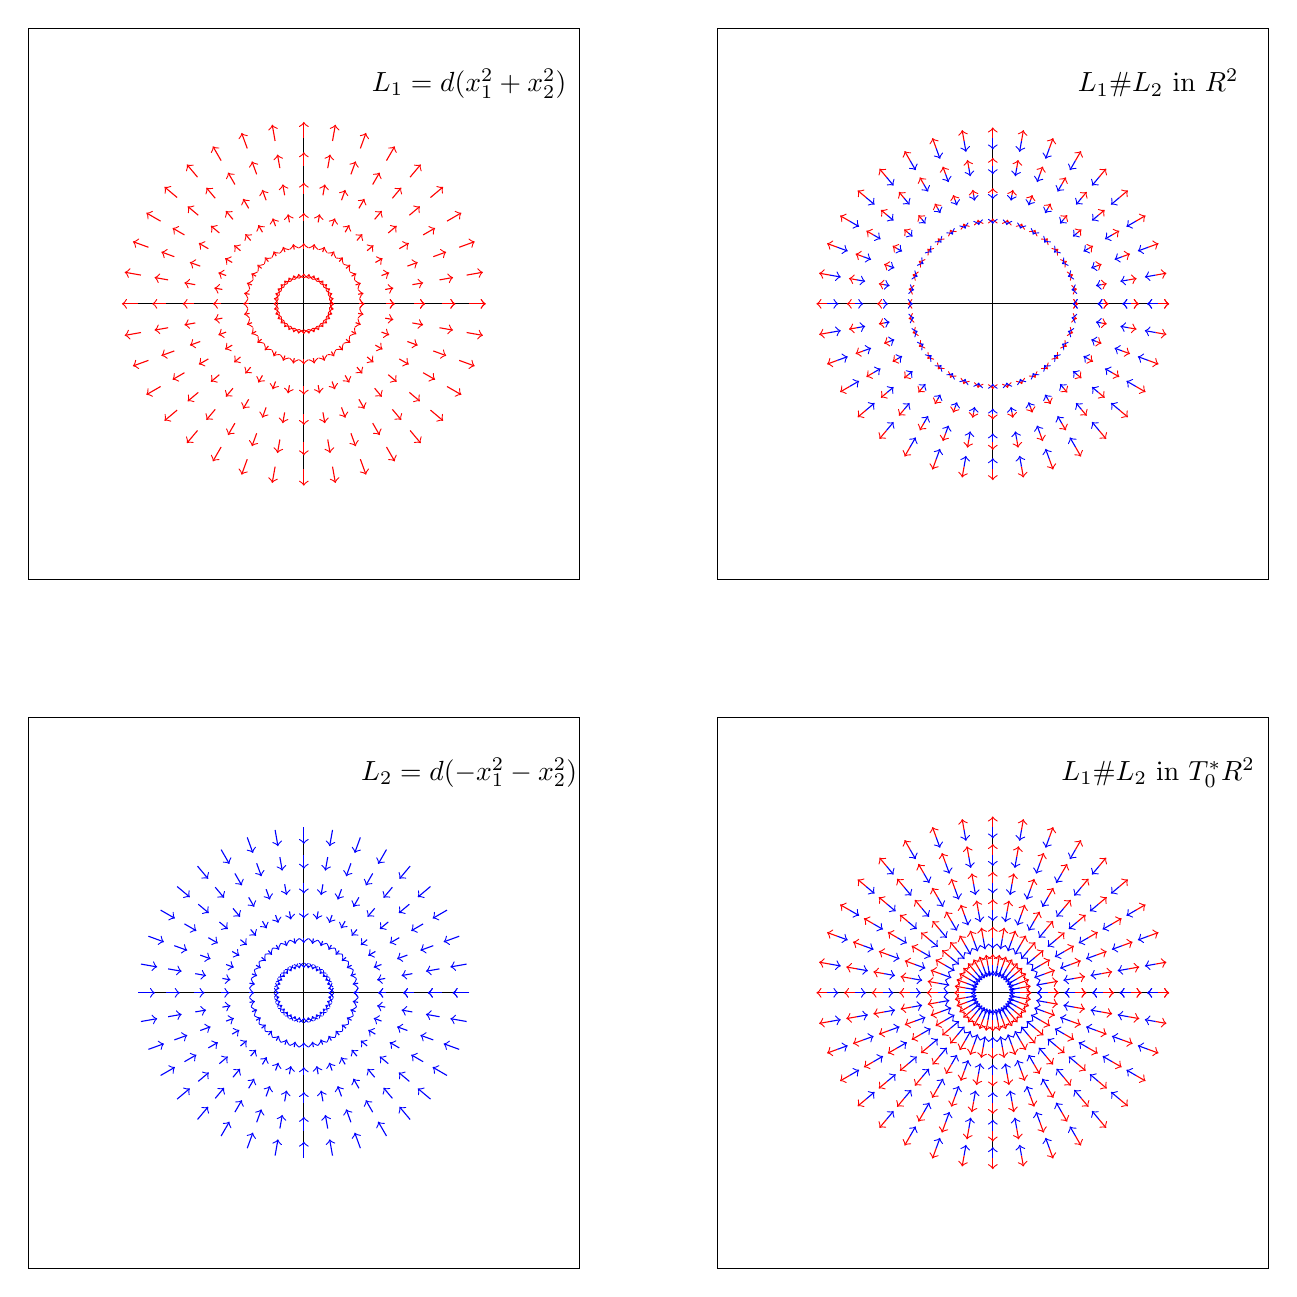
\begin{tikzpicture}[scale=.7]


    \begin{scope}[shift={(-12.5,1)}]
    \draw  (-5,5) rectangle (5,-5);
    \node at (3,4) {$L_1= d(x^2_1+x_2^2)$};
    
    \begin{scope}
    \draw (-3,0)--(3,0) (0,3)--(0,-3);
    \foreach \r in { .5, 1,1.5, 2,2.5, 3} {
        \foreach \t in {0,...,36} {
            \draw[->, red] ({\r * cos(10*\t)},{ \r * sin(10*\t) })-- ({1.1*\r * cos(10*\t)},{ 1.1*\r * sin(10*\t) });
            %\draw[->, blue] ({\r * cos(10*\t)},{ \r * sin(10*\t) })-- ({0.9*\r * cos(10*\t)},{ 0.9*\r * sin(10*\t) });
        }
    }
    \end{scope}
    \end{scope}
    
    
    \begin{scope}[shift={(-12.5,-11.5)}]
    
    
    \draw  (-5,5) rectangle (5,-5);
    
    \node at (3,4) {$L_2=d(-x^2_1-x_2^2)$};
        \begin{scope}
    \draw (-3,0)--(3,0) (0,3)--(0,-3);
    \foreach \r in { .5, 1,1.5, 2,2.5, 3} {
        \foreach \t in {0,...,36} {
            %\draw[->, red] ({\r * cos(10*\t)},{ \r * sin(10*\t) })-- ({1.1*\r * cos(10*\t)},{ 1.1*\r * sin(10*\t) });
            \draw[->, blue] ({\r * cos(10*\t)},{ \r * sin(10*\t) })-- ({0.9*\r * cos(10*\t)},{ 0.9*\r * sin(10*\t) });
        }
    }
    \end{scope}
    \end{scope}
    
    \begin{scope}[]
    
    \begin{scope}[shift={(0,1)}]
    
    
    \draw  (-5,5) rectangle (5,-5);
    
    \node at (3,4) {$L_1\#L_2$ in $\mathbb R^2$};
    
    
    
    \begin{scope}
    \draw (-3,0)--(3,0) (0,3)--(0,-3);
    \foreach \r in { .5, 1,1.5, 2} {
        \foreach \t in {0,...,36} {
            \draw[->, red] ({(\r+1) * cos(10*\t)},{ (\r+1) * sin(10*\t) })-- ({(1.1*\r +1)* cos(10*\t)},{ (1.1*\r+1) * sin(10*\t) });
            \draw[->, blue] ({(\r+1) * cos(10*\t)},{ (\r+1) * sin(10*\t) })-- ({(0.9*\r+1) * cos(10*\t)},{( 0.9*\r +1)* sin(10*\t) });
        }
    }
    \end{scope}
    \end{scope}
    \begin{scope}[shift={(0,-11.5)}]
    
    
    \draw  (-5,5) rectangle (5,-5);
    
    \node at (3,4) {$L_1\#L_2$ in $T^*_0\mathbb R^2$};
    
    \begin{scope}
    \draw (-3,0)--(3,0) (0,3)--(0,-3);
    \foreach \r in {.5, 1,1.5, 2,2.5, 3} {
        \foreach \t in {0,...,36} {
            \draw[->, red] ({\r * cos(10*\t)},{ \r * sin(10*\t) })-- ({(\r+.2) * cos(10*\t)},{ (\r+.2) * sin(10*\t) });
            \draw[->, blue] ({\r * cos(10*\t)},{ \r * sin(10*\t) })-- ({(\r-.2) * cos(10*\t)},{ (\r-.2) * sin(10*\t) });
        }
    }
    \end{scope}
    \end{scope}
    
    \end{scope}
    
    \end{tikzpicture}